% D4 - The Kappa Replay & Reprocessing Mechanism
\documentclass[border=8pt]{standalone}
% Shared styling for every Kappa report diagram.
%
% Colour convention across diagrams:
%   BLUE       stream path     - unified streaming engine and message broker
%   GREEN      storage layer   - query-first Cassandra tables and master log
%   ORANGE     serving layer   - low-latency FastAPI endpoints
%   RED        clinical alerts - acute deterioration notifications
%   GREY       infrastructure  - orchestrators, metrics and supporting daemons
%
% TikZ rather than raster graphics ensures vector resolution and matching typography.

\usepackage{amsmath}
\usepackage{tikz}
\usepackage{xcolor}
\usetikzlibrary{positioning,arrows.meta,fit,backgrounds,calc,shapes.geometric,decorations.pathreplacing}

\definecolor{streamblue}{HTML}{0078D7}
\definecolor{streambg}{HTML}{E6F2FB}
\definecolor{storegreen}{HTML}{2E7D4A}
\definecolor{storebg}{HTML}{E4F3E8}
\definecolor{servorange}{HTML}{C2660A}
\definecolor{servbg}{HTML}{FCEDDD}
\definecolor{alertred}{HTML}{D83B01}
\definecolor{alertbg}{HTML}{FDE7E9}
\definecolor{infragrey}{HTML}{5A6672}
\definecolor{infrabg}{HTML}{ECEFF1}
\definecolor{edgegrey}{HTML}{444C54}

\tikzset{
  box/.style={
    draw, rounded corners=2pt, align=center, inner sep=5pt,
    font=\scriptsize, minimum height=8mm, line width=0.5pt,
  },
  stream/.style={box, draw=streamblue, fill=streambg, text=black},
  store/.style ={box, draw=storegreen, fill=storebg,  text=black},
  serv/.style  ={box, draw=servorange, fill=servbg,   text=black},
  alert/.style ={box, draw=alertred,   fill=alertbg,  text=black},
  infra/.style ={box, draw=infragrey,  fill=infrabg,  text=black},
  ext/.style   ={box, draw=edgegrey,   fill=white, dashed, text=black},
  cqlbox/.style={
    draw=storegreen, fill=white, rounded corners=1.5pt,
    align=left, inner sep=3pt, font=\tiny, line width=0.4pt
  },
  flow/.style  ={-{Stealth[length=4pt]}, draw=edgegrey, line width=0.5pt},
  streamflow/.style={flow, draw=streamblue, line width=0.7pt},
  alertflow/.style={flow, draw=alertred, line width=0.7pt},
  lbl/.style   ={font=\tiny\itshape, text=edgegrey, fill=white, inner sep=1.5pt},
  zone/.style  ={draw=edgegrey, dashed, rounded corners=3pt, line width=0.4pt, inner sep=7pt},
  ztitle/.style={font=\scriptsize\bfseries, text=edgegrey, fill=white, inner xsep=3pt, inner ysep=1pt},
}

\begin{document}
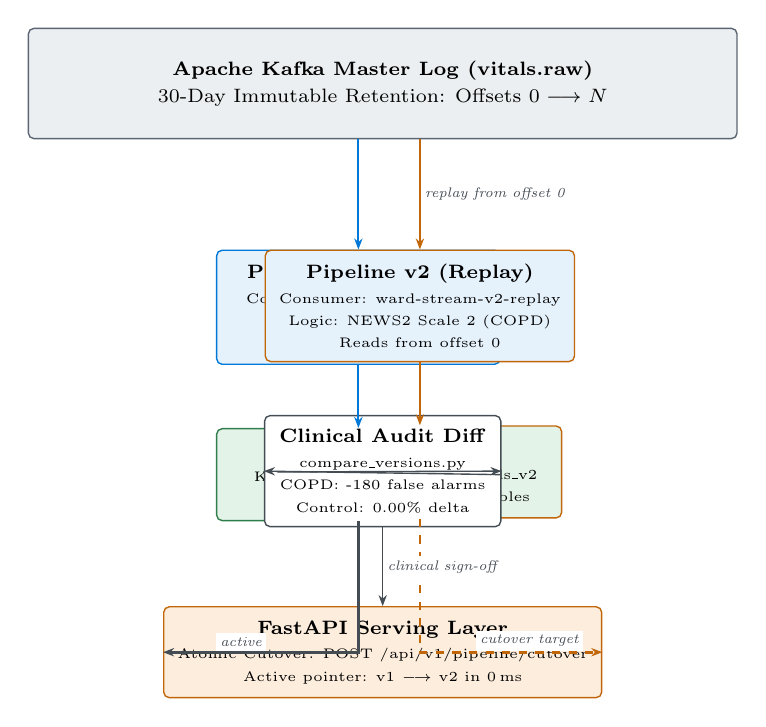
\begin{tikzpicture}[node distance=7mm]

% Kafka log
\node[infra, minimum width=90mm, minimum height=14mm] (log)
  {\textbf{Apache Kafka Master Log (vitals.raw)}\\[2pt]\scriptsize 30-Day Immutable Retention: Offsets $0 \longrightarrow N$};

% Active pipeline v1
\node[stream, below left=14mm and -15mm of log.south, minimum width=36mm] (v1)
  {\textbf{Pipeline v1 (Active)}\\[1pt]\tiny Consumer: ward-stream-v1\\\tiny Logic: NEWS2 Scale 1\\\tiny Reads at log head};

\node[store, below=8mm of v1, minimum width=36mm] (c1)
  {\textbf{Cassandra (v1)}\\[1pt]\tiny Keyspace: hospital\_vitals\\\tiny Active serving tables};

% Replay pipeline v2
\node[stream, below right=14mm and -15mm of log.south, minimum width=36mm, draw=servorange] (v2)
  {\textbf{Pipeline v2 (Replay)}\\[1pt]\tiny Consumer: ward-stream-v2-replay\\\tiny Logic: NEWS2 Scale 2 (COPD)\\\tiny Reads from offset 0};

\node[store, below=8mm of v2, minimum width=36mm, draw=servorange] (c2)
  {\textbf{Cassandra (v2)}\\[1pt]\tiny Keyspace: hospital\_vitals\_v2\\\tiny Parallel reprocessed tables};

% Comparator / Audit
\node[box, draw=edgegrey, fill=white, below=10mm of log, yshift=-25mm, minimum width=30mm] (diff)
  {\textbf{Clinical Audit Diff}\\[1pt]\tiny compare\_versions.py\\\tiny COPD: -180 false alarms\\\tiny Control: 0.00\% delta};

% Serving layer cutover
\node[serv, below=10mm of diff, minimum width=45mm] (api)
  {\textbf{FastAPI Serving Layer}\\[1pt]\tiny Atomic Cutover: POST /api/v1/pipeline/cutover\\\tiny Active pointer: v1 $\longrightarrow$ v2 in 0\,ms};

% Edges
\draw[streamflow] (log.south -| v1.north) -- (v1.north);
\draw[streamflow, draw=servorange] (log.south -| v2.north) -- node[lbl, right] {replay from offset 0} (v2.north);

\draw[streamflow] (v1) -- (c1);
\draw[streamflow, draw=servorange] (v2) -- (c2);

\draw[flow] (c1.east) -- (diff.west);
\draw[flow] (c2.west) -- (diff.east);

\draw[flow, line width=1pt] (c1.south) |- node[lbl, pos=0.8, above] {active} (api.west);
\draw[flow, dashed, line width=1pt, draw=servorange] (c2.south) |- node[lbl, pos=0.8, above] {cutover target} (api.east);

\draw[flow] (diff.south) -- node[lbl, right] {clinical sign-off} (api.north);

\end{tikzpicture}
\end{document}
